\chapter{Theoretical Motivations
\label{ch:theory}}

%\setcounter{section}{-1}

\section{The Standard Model}

The standard model (SM) of particle physics includes three fundamental forces and all of the particles of ordinary matter using a locally gauge-invariant quantum field theory framework. The three fundamental forces are electromagnetism, the weak force, and the strong force. These forces are carried by spin-1 gauge bosons, while the matter particles consist of quarks and leptons, two categories of spin-1/2 fermions. When these forces are weak enough, quantum field theory calculations use a perturbative method in which the leading order (LO) term is calculated, then the next-to-leading order (NLO) correction is added, then the next-to-next-to-leading order correction (NNLO), and so forth. In addition, the standard model contains a scalar spin-0 boson, the Higgs boson, which is part of the Higgs field that provides masses to certain gauge bosons and fermions. Figure \ref{fig:sm-particles} summarizes the particles in the standard model, including the spin, electric charge, and mass values of each particle. The standard model and quantum field theory are described in more detail in many standard textbooks.

\begin{figure}[hbt]
\begin{center}
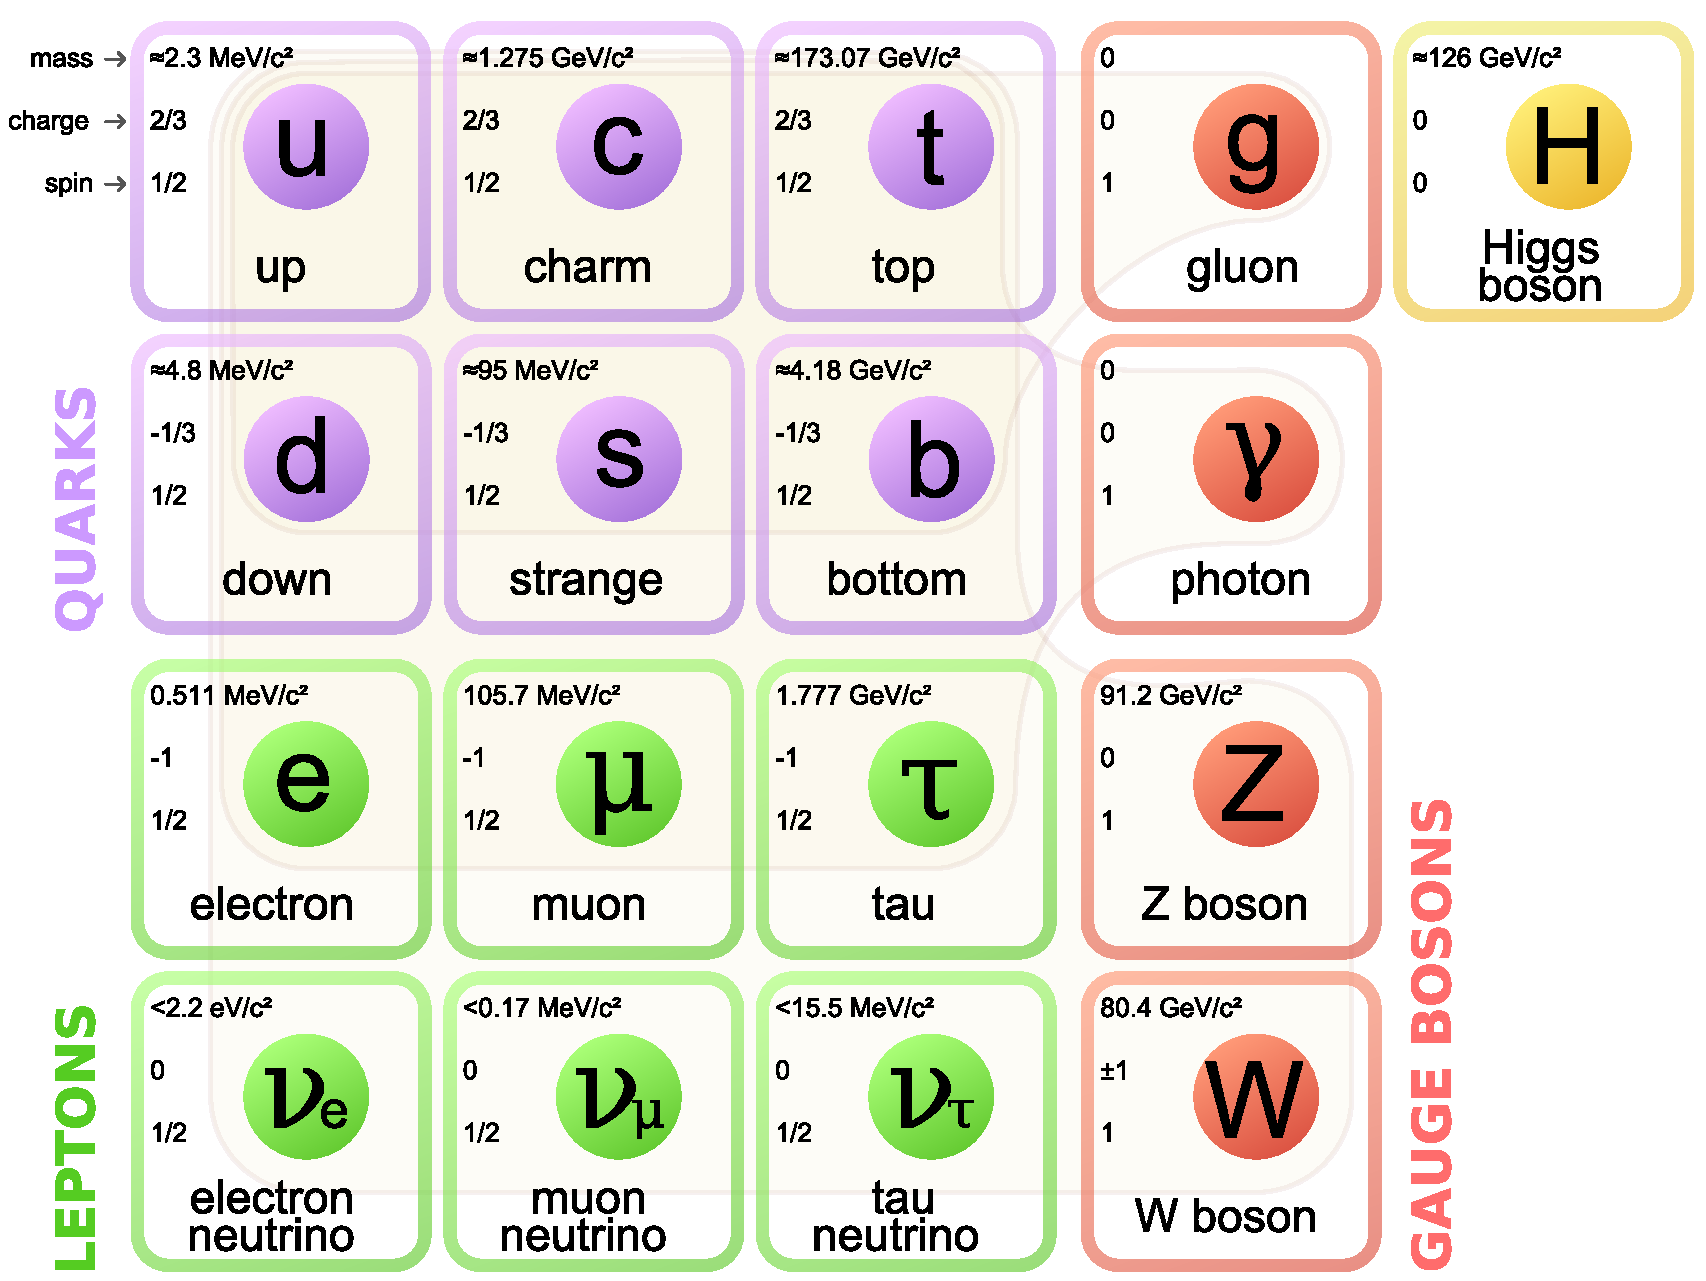
\includegraphics[width=0.95\textwidth]{figures/Standard_Model_of_Elementary_Particles.pdf}
\caption{A table of all the elementary particles in the standard model, with the spin, electric charge, and mass values of each particle \cite{MissMJ}. The faint gray lines indicate which gauge bosons interact with which fermions.}
\label{fig:sm-particles}
\end{center}
\end{figure}

The electromagnetic force is mediated by photons ($\gamma$), spin-1 gauge bosons which have no mass or electric charge $Q$. This force causes interactions between electrically charged particles and has infinite range due to the masslessness of the photon. Quantum electrodynamics (QED) is a gauge-invariant quantum field theory embedding a $U(1)$ symmetry group that describes electromagnetism. The weak force is mediated by the massive \Wpm and \Z bosons and can be represented by an $SU(2)$ symmetry group. The weak force acts on particles carrying weak isospin $T$. Weak isospin is a quantum number whose third component $T_3$ is conserved in all interactions and which has the same mathematical group structure as angular momentum, though the two quantities are physically distinct. The massiveness of the weak carrier bosons means that the weak force has a limited range, approximately $10^{-18}\unit{m}$. The charged current weak interaction, mediated by the \Wpm bosons, is sensitive to the chirality of fermions; only left-handed fermions and right-handed antifermions participate in this interaction. The neutral current weak interaction, mediated by the \Z boson, acts on fermions of all chiralities, with different coupling strengths depending on the chirality.

As suggested by the inclusion of both forces in the previous paragraph, the electromagnetic and weak forces can be unified to form the electroweak force, represented by the symmetry group $SU(2)_{L} \times U(1)_{Y}$. In this unification, the quantum numbers of electromagnetism and the weak force are related by a new conserved quantum number, weak hypercharge $Y = 2(Q - T_3)$. The Higgs mechanism is responsible for electroweak symmetry breaking (EWSB). In order for the electroweak theory to be gauge invariant, the gauge bosons must be massless, but the \Wpm and \Z bosons are observed to have mass. The Higgs mechanism solves this dilemma via spontaneous EWSB due to its non-zero vacuum expectation value (VEV). The Higgs field consists of a doublet, with two charged particles and two neutral particles, all scalar bosons. The two charged particles and one of the neutral particles act as Goldstone bosons, combining with the \Wpm and \Z bosons to produce their masses. The remaining neutral particle is the Higgs boson, which was discovered at the LHC in 2012 \cite{NewBoson}.

The strong force, quantum chromodynamics (QCD), is mediated by gluons (\cPg) and can be represented by an $SU(3)$ symmetry group. Gluons, like photons, are spin-1 gauge bosons without mass or electric charge. However, gluons do possess color charge, the quantum number on which the strong force acts. Color charge is so named because the charge has three possible values, which are labeled red, green, or blue. The strong force between quarks does not decrease as they become spatially separated, a phenomenon known as confinement. The energy in the gluon field between the separated quarks can become large enough to form one or more quark-antiquark pairs, which prevents quarks or gluons from existing in a bare state. Correspondingly, the range of the strong force is limited to ${\sim} 10^{-15}\unit{m}$. Quarks and gluons are always observed in nature as bound states called hadrons, and the formation of those bound states is called hadronization. States with one quark and one antiquark are mesons, while states with three quarks are baryons. Mesons and baryons are the two allowed types of bound states because they represent color singlets. Complementarily, as quarks get closer together, the strong force between them weakens. This behavior is known as asymptotic freedom; because short distances are equivalent to high energies, the strong interactions of quarks at a high-energy collider like the LHC can be calculated perturbatively. A residual form of the strong force acts on nucleons, protons and neutrons, to form atomic nuclei.

As mentioned, fermions are the particles of matter, which are separated into two groups: quarks and leptons. Quarks have fractional electric charge, weak isospin, and color charge, so they are affected by all three fundamental forces. There are two types of quarks: up-type quarks that have $Q = 2/3$ and down-type quarks that have $Q = -1/3$. Leptons consist of charged leptons and neutrinos. Charged leptons possess electric charge and weak isospin, while neutrinos only possess weak isospin. In total, there are six flavors of leptons and six flavors of quarks, arranged into three generations. The flavors of up-type quarks are the up, charm, and top quarks; the flavors of down-type quarks are the down, strange, and bottom quarks; the flavors of charged leptons are the electron, muon, and tau lepton; and the flavors of the neutrinos are the electron, muon, and tau neutrinos. The top quark is the heaviest elementary particle and is so heavy that it decays before hadronizing, making it an exception to the rule that quarks are only observed in bound states. Quarks possess an additively conserved quantum number called baryon number $B$, which is defined as $B = \frac{1}{3}(n_{\cPq} - n_{\overline{\cPq}})$. The conservation of baryon number results in the stability of the proton, as it is the lightest baryon. Similarly, lepton number $L$ is defined for leptons as $L = n_{\ell} - n_{\overline{\ell}}$. Specific lepton flavor numbers $L_{\Pe}$, $L_{\mu}$, $L_{\tau}$ are defined for each flavor pair of leptons. Baryon number and lepton number are accidental symmetries of the standard model, as only higher-dimensional terms excluded from the SM Lagrangian would break them. 

The fermions are arranged into multiplets based on their chirality. The left-handed up- and down-type quarks are grouped together in a weak doublet $\cPq_L$, as are the left-handed charged leptons and neutrinos in $\ell_L$. The right-handed particles are weak singlets. It is important to note that right-handed neutrinos, and correspondingly left-handed antineutrinos, do not exist in the standard model. The Higgs field spontaneously provides masses to the quarks and charged leptons through a Yukawa interaction which couples the left- and right-handed versions of each flavor of particle. For a fermion $f$, this interaction takes the form $-y_{f} \overline{f}_{L} \PH f_{R}$, where $y_{f}$ is the Yukawa coupling. The mass eigenstates formed by this interaction are mixtures of the weak eigenstates, leading to flavor-changing charged weak currents for the quarks, with the amount of mixing between any two flavors given by the unitary Cabibbo-Kobayashi-Maskawa (CKM) matrix. The quantum numbers of each type of particle are summarized in Table \ref{tab:q-num}, and the interactions among all the particles are illustrated in Fig. \ref{fig:sm-interactions}.

\begin{table}[htb]
  \begin{center}
%    \def\arraystretch{2.0} %1 is the default
    \begin{tabular}{|l||l|r|r|r|r|r|}
\hline
      & \multicolumn{1}{c|}{Particle} & \multicolumn{1}{c|}{$Q$} & \multicolumn{1}{c|}{$T_3$} & \multicolumn{1}{c|}{$Y$} & \multicolumn{1}{c|}{$B$} & \multicolumn{1}{c|}{$L$} \\
\hline
\hline
\multirow{3}{*}{Quarks}  
\rule{0pt}{24pt}         & $\cPq_L = \doublet[r]{\cPqu}{\cPqd}_L$ & $\doublet[r]{2/3}{-1/3}$ & $\doublet[r]{1/2}{-1/2}$ & $1/3$  & $1/3$ & 0 \\
                         & $\cPqu_R$                              & $2/3\hphantom{\bigg)}$   & $0\hphantom{\bigg)}$     & $4/3$  & $1/3$ & 0 \\
                         & $\cPqd_R$                              & $-1/3\hphantom{\bigg)}$  & $0\hphantom{\bigg)}$     & $-2/3$ & $1/3$ & 0 \\
\hline
\hline
\multirow{2}{*}{Leptons} 
\rule{0pt}{24pt}         & $\ell_L = \doublet[r]{\nu}{\Pe}_L$     & $\doublet[r]{0}{-1}$     & $\doublet[r]{1/2}{-1/2}$ & $-1$   & 0     & 1 \\
                         & $\Pe_R$                                & $-1\hphantom{\bigg)}$    & $0\hphantom{\bigg)}$     & $-2$   & 0     & 1 \\
\hline
    \end{tabular}
    \caption{The quantum numbers of each category of fermions, based on chirality and particle type: up-type quarks, down-type quarks, charged leptons, and neutrinos. The various flavors of each category, also called the first, second, and third generations of matter, possess the same quantum numbers and differ only in their masses.}
    \label{tab:q-num}
  \end{center}
\end{table}

\begin{figure}[hbt]
\begin{center}
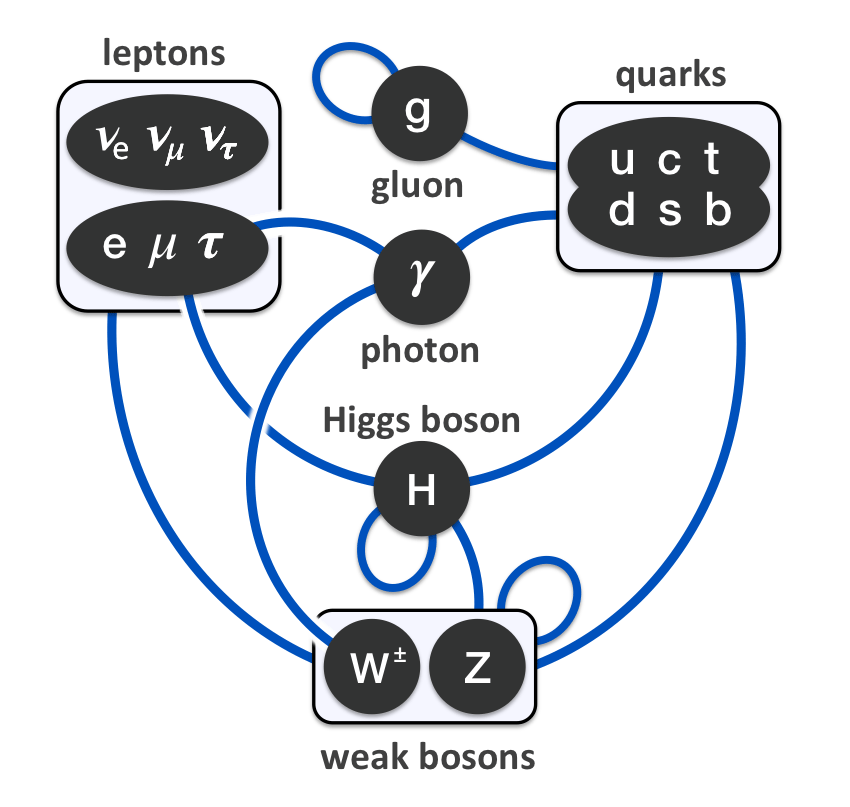
\includegraphics[width=0.95\textwidth]{figures/Elementary_particle_interactions_in_the_Standard_Model.png}
\caption{A diagram illustrating the leading order interactions between particles in the standard model, including self-interactions \cite{Drexler}.}
\label{fig:sm-interactions}
\end{center}
\end{figure}

%\addtocounter{section}{-1}
%\renewcommand{\thesection}{\thechapter.{$\frac{1}{2}$}}
\section{Beyond the Standard Model}
%\newcounter{sectionprime}
%\addtocounter{sectionprime}{\value{section}}
%\addtocounter{sectionprime}{-1}
%\renewcommand{\thesection}{\thechapter.\arabic{sectionprime}} % use offset numbering

The predictions of the standard model have been confirmed by decades of precise experimental tests. However, as an effective field theory, its domain of applicability is ultimately limited; at a high enough energy, the theory will break down. Further, some laboratory and cosmological observations are difficult to accommodate in the standard model. These limitations and indications of new phenomena, as well as aesthetic considerations, motivate various searches for physics beyond the standard model (BSM), including the searches which will be presented in this dissertation.

Electroweak unification and charge quantization suggest that a Grand Unified Theory (GUT) could unify all three fundamental forces, at an expected energy scale of ${\sim} 10^{16}\GeV$ \cite{PhysRevLett.33.451}. The observation of neutrino oscillations is now well established, indicating that neutrinos have small but non-zero masses. The oscillation of neutrinos between mass and flavor eigenstates is described by the Pontecorvo-Maki-Nakagawa-Sakata (PMNS) matrix. The PMNS matrix is unitary and has four parameters: three mixing angles and one phase, similar to the CKM matrix for quarks. The values of the neutrino masses have not been directly measured, but are indirectly limited to the \eVns scale. Because right-handed neutrinos do not exist in the Standard Model, neutrinos cannot gain mass via a Yukawa interaction with the Higgs field.

Though the Higgs mass is a parameter of the SM, it can be calculated in many BSM theories \cite{Susskind1984181}. Unless unnatural fine-tuning occurs, this calculation produces a value near the Planck scale of $10^{19}\GeV$, orders of magnitude higher than the observed value of 125\GeV, which characterizes the electroweak scale. This is known as the hierarchy problem. To construct a natural theory which avoids such fine-tuning while making predictions that agree with observation, it is necessary to cancel divergent contributions to the Higgs mass. The hierarchy problem is an important motivation to search for new physics at the LHC \cite{Morrissey20121}.

Astrophysics provides numerous indications of the need for BSM theories. Most notably, the measurement of galactic rotation curves and galaxy cluster collisions \cite{BulletCluster} indicates that dark matter makes up ${\sim} 85\%$ of the matter in the universe. Dark matter interacts gravitationally but not electromagnetically or strongly; it is currently unknown if dark matter interacts weakly. Dark matter is likely to be a new particle not present in the standard model. The most popular type of dark matter candidate is a weakly interacting massive particle (WIMP) \cite{Morrissey20121}, but many other candidates have been proposed \cite{PDG}.

Gravity is not included in the standard model. A successful unification of general relativity and quantum field theory has not been achieved, due to the difficulty of constructing a renormalizable theory for the spin-2 graviton. At the Planck scale, gravitational effects become comparable to SM interactions, which calls for a new theory.

The following sections discuss the theories of leptoquarks and R-parity violating supersymmetry. The existence of leptoquarks can be a consequence of grand unification or other theories that address the parallels between leptons and quarks in the standard model. Supersymmetry is motivated by basic considerations of quantum field theory, the hierarchy problem, grand unification, and dark matter \cite{SUSY1,SUSY2}. The introduction of R-parity violation in supersymmetry evades existing limits on signatures with large missing transverse energy due to the stability of the lightest supersymmetric particle (LSP). Without a stable LSP, R-parity violating supersymmetry lacks a dark matter candidate. However, it retains other desirable characteristics of supersymmetry, including a solution to the hierarchy problem and grand unification. R-parity violating supersymmetry can also act as a signature generator to suggest novel searches which might discover or rule out other BSM theories \cite{EvansSigGen}.

%\stepcounter{sectionprime}
\section{Leptoquarks
\label{sec:LQ}}

Many BSM theories include a deeper relationship between leptons and quarks. Such a relationship is indicated by the cancellation of SM gauge anomalies from triangle diagrams, which requires each generation of matter to consist of quarks and leptons with the specific weak hypercharge values and multiplet arrangements that they possess in the SM \cite{Peskin}. Such theories introduce a class of particles called leptoquarks (LQs), which possess lepton number, baryon number, color charge, and fractional electric charge. Leptoquarks are bosons, either scalar with spin 0 or vector with spin 1. The values of the LQ quantum numbers are model-dependent. A total fermion number $F$ can be defined as $F = 3B + L$ to characterize the combinations of lepton and baryon numbers found in LQs. The possible values are $F=0$ for LQs which couple to $\overline{\ell}\cPq$ or $\ell\overline{\cPq}$ pairs and $|F|=2$ for coupling to $\ell\cPq$ or $\overline{\ell}\overline{\cPq}$ pairs.

In general, grand unified theories group leptons and quarks together in multiplets. The first BSM theory to include leptoquarks was the $SU(4)$ model by Pati and Salam \cite{SU4}, a GUT which casts lepton number as the fourth type of color charge, hence the $SU(4)$ symmetry instead of the SM $SU(3)$. Another GUT, the $SU(5)$ model by Georgi and Glashow \cite{GUT}, also contains leptoquarks. However, the symmetries in these theories are typically assumed to break at the GUT scale, rendering the expected LQ masses very large and therefore unable to be directly produced at colliders. $E_6$ superstring theory \cite{SUPERSTR} can also contain LQs, as it behaves similarly to GUTs below the string compactification scale, which is typically near the Planck scale. In other models, leptoquarks may be composite particles \cite{LQ3b}. These include extended technicolor theories \cite{TC3}, which postulate a new strong interaction similar to QCD, and provide spontaneous masses to SM fermions using technifermions. A techniquark and anti-technilepton can bind together to form a technimeson which interacts with SM fermions as a leptoquark with a model-dependent coupling. Technicolor, though, has become disfavored after experimental data confirmed the Higgs mechanism as the solution to EWSB and spontaneous fermion masses.

The Buchm\"{u}ller-R\"{u}ckl-Wyler (BRW) model of leptoquarks includes all renormalizable Lagrangian terms compatible with the standard model \cite{BRW}. There are several constraints imposed in the BRW model:
\begin{enumerate}
\item LQ interactions are dimensionless, in order to be renormalizable.
\item LQ interactions are invariant under the overall SM symmetry \linebreak[4] ${SU(3)_{C} \times SU(2)_{L} \times U(1)_{Y}}$.
\item LQ interactions conserve $B$ and $L$, to avoid contributions to proton decay.
\item LQs couple only to SM particles.
\end{enumerate}
Further consideration of experimental limits imposes two additional constraints, creating the minimal BRW (mBRW) model:
\begin{enumerate}
\setcounter{enumi}{4}
\item LQ couplings are chiral, involving either only left-handed fermions or only right-handed fermions, due to limits on otherwise chirally-suppressed decays such as $\pi^{+} \rightarrow \Pe^{+} \nu_{\Pe}$.
\item LQ couplings involve only a single generation of leptons and quarks, to evade limits on flavor-changing neutral currents (FCNCs).
\end{enumerate}
The Lagrangian terms are given for scalar LQs in Eq. \eqref{eq:Lagrangian-SLQ} and for vector LQs in Eq. \eqref{eq:Lagrangian-VLQ} below, using the ``Aachen'' notation as specified in Ref. \cite{ModelIndLQ}.
\begin{align}
\label{eq:Lagrangian-SLQ}
\mathcal{L}_{S} = &\hphantom{+~}(\lambda_{L,S_{0}} \overline{\cPq}_{L}^{c} i\sigma_{2} \ell_{L} + \lambda_{R,S_{0}} \overline{\cPqu}_{R}^{c} \Pe_{R})S_{0}^{\dagger}
+ \lambda_{R,\widetilde{S}_{0}} \overline{\cPqd}_{R}^{c} \Pe_{R} \widetilde{S}_{0}^{\dagger} \nonumber \\
&+ (\lambda_{L,S_{1/2}} \overline{\cPqu}_{R} \ell_{L} + \lambda_{R,S_{1/2}} \overline{\cPq}_{L} i\sigma_{2} \Pe_{R})S_{1/2}^{\dagger}
+ \lambda_{L,\widetilde{S}_{1/2}} \overline{\cPqd}_{R} \ell_{L} \widetilde{S}_{1/2}^{\dagger} \nonumber \\
&+ \lambda_{L,S_{1}} \overline{\cPq}_{L}^{c} i\sigma_{2}\boldsymbol{\sigma} \ell_{L} \cdot \boldsymbol{S}_{1}^{\dagger} + \text{h.c.} \\
%\end{align}
%\begin{align}
\label{eq:Lagrangian-VLQ}
\mathcal{L}_{V} = &\hphantom{+~}(\lambda_{L,V_{0}} \overline{\cPq}_{L} \gamma_{\mu} \ell_{L} + \lambda_{R,V_{0}} \overline{\cPqd}_{R} \gamma_{\mu} \Pe_{R})V_{0}^{\mu\dagger}
+ \lambda_{R,\widetilde{V}_{0}} \overline{\cPqu}_{R} \gamma_{\mu} \Pe_{R} \widetilde{V}_{0}^{\mu\dagger} \nonumber \\
&+ (\lambda_{L,V_{1/2}} \overline{\cPqd}_{R}^{c} \gamma_{\mu} \ell_{L} + \lambda_{R,V_{1/2}} \overline{\cPq}_{L}^{c} \gamma_{\mu} \Pe_{R})V_{1/2}^{\mu\dagger}
+ \lambda_{L,\widetilde{V}_{1/2}} \overline{\cPqu}_{R}^{c} \gamma_{\mu} \ell_{L} \widetilde{V}_{1/2}^{\mu\dagger} \nonumber \\
&+ \lambda_{L,V_{1}} \overline{\cPq}_{L} \gamma_{\mu}\boldsymbol{\sigma} \ell_{L} \cdot \boldsymbol{V}_{1}^{\mu\dagger} + \text{h.c.}
\end{align}
In these equations, scalar leptoquarks are denoted by $S$ and vector leptoquarks are denoted by $V$. The subscripts 0, 1/2, and 1 denote singlet, doublet, and triplet states, respectively. Similar states with different quantum numbers are separated in the notation by the presence or absence of a tilde $\widetilde{\phantom{S}}$. The coupling constants for the Yukawa couplings between leptoquarks, leptons, and quarks are represented by $\lambda$, with the chirality $L$ or $R$ and the leptoquark type indicated in the subscript. The generation indices for the couplings and fermion multiplets are suppressed. The Pauli matrices are denoted by $\sigma_{i}$ and the Dirac matrices by $\gamma_{\mu}$. The Hermitian conjugate terms are indicated as ``h.c.'' The quantum numbers for the different types of mBRW leptoquarks are listed in Table \ref{tab:lq-num}.

\begin{table}[htb]
  \begin{center}
%    \def\arraystretch{3.0} %1 is the default
    \begin{tabular}{|l||l|r|r|r|r|}
\hline
      & \multicolumn{1}{c|}{Particle} & \multicolumn{1}{c|}{$Q$} & \multicolumn{1}{c|}{$T_3$} & \multicolumn{1}{c|}{$Y$} & \multicolumn{1}{c|}{$F$} \\
\hline
\hline
\multirow{10}{*}{Scalar} & $S_{0}$               & $-1/3\hphantom{\bigg)}$                            & $0\hphantom{\bigg)}$                              & $-2/3$ & $2$ \\
                         & $\widetilde{S}_{0}$   & $-4/3\hphantom{\bigg)}$                            & $0\hphantom{\bigg)}$                              & $-8/3$ & $2$ \\
\rule{0pt}{24pt}         & $S_{1/2}$             & $\doublet[r]{-2/3}{-5/3}$ & $\doublet[r]{1/2}{-1/2}$ & $-7/3$ & $0$ \\
\rule{0pt}{24pt}         & $\widetilde{S}_{1/2}$ & $\doublet[r]{1/3}{-2/3}$  & $\doublet[r]{1/2}{-1/2}$ & $-1/3$ & $0$ \\
\rule{0pt}{36pt}         & $S_{1}$               & $\triplet[r]{2/3}{-1/3}{-4/3}$       & $\triplet[r]{1\vphantom{/}}{0\vphantom{/}}{-1\vphantom{/}}$             & $-2/3$ & $2$ \\
\hline
\hline
\multirow{10}{*}{Vector} & $V_{0}$               & $-2/3\hphantom{\bigg)}$                            & $0\hphantom{\bigg)}$                              & $-4/3$  & $0$ \\
                         & $\widetilde{V}_{0}$   & $-5/3\hphantom{\bigg)}$                            & $0\hphantom{\bigg)}$                              & $-10/3$ & $0$ \\
\rule{0pt}{24pt}         & $V_{1/2}$             & $\doublet[r]{-1/3}{-4/3}$ & $\doublet[r]{1/2}{-1/2}$ & $-5/3$  & $2$ \\
\rule{0pt}{24pt}         & $\widetilde{V}_{1/2}$ & $\doublet[r]{2/3}{-1/3}$  & $\doublet[r]{1/2}{-1/2}$ & $1/3$   & $2$ \\
\rule{0pt}{36pt}         & $V_{1}$               & $\triplet[r]{1/3}{-2/3}{-5/3}$       & $\triplet[r]{1\vphantom{/}}{0\vphantom{/}}{-1\vphantom{/}}$             & $-4/3$  & $0$ \\
\hline
    \end{tabular}
    \caption{The quantum numbers of the different types of scalar and vector leptoquarks in the mBRW model.}
    \label{tab:lq-num}
  \end{center}
\end{table}

As color-charged particles, leptoquarks are primarily produced by strong interactions in $\Pp\Pp$ collisions. For pair production of leptoquarks, these interactions include gluon-gluon fusion and quark-antiquark annihilation, whose LO Feynman diagrams are shown in Fig. \ref{fig:lq-diagrams}. An additional contribution to quark-antiquark annihilation may proceed through the Yukawa coupling $\lambda$ of the leptoquark to the quark and lepton pair. However, the ratio $\MLQ/\lambda$, where $\MLQ$ is the leptoquark mass, is restricted by limits from low-energy processes including $\pi^{+} \rightarrow \Pe^{+} \nu_{\Pe}$ and atomic parity violation. The limits on $\MLQ/\lambda$ range from 1800--6400\GeVcc, depending on the type of leptoquark \cite{Leurer:1993em, MuchAdo, LQreview}. The expected accessible mass range for leptoquarks at the LHC with $\sqrt{s}=14\TeV$ ranges from 900--1200\GeVcc for scalar LQs and 1200--1500\GeVcc for vector LQs, depending on the desired number of events \cite{LQPairHad}. Up to these masses, $\lambda$ will be small enough that its contribution to leptoquark production can be neglected. This applies both to the Yukawa-based pair production diagram in Fig. \ref{fig:lq-diagrams} and the single production diagrams from quark-gluon scattering in Fig. \ref{fig:lq-single}.

\begin{figure}[hbt]
\begin{center}
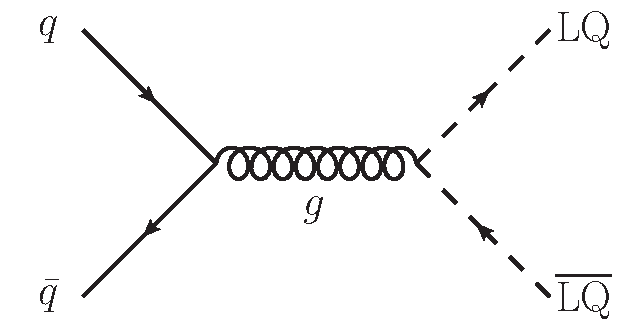
\includegraphics[width=0.49\textwidth]{figures/LO_FD_LQ_pair_a.pdf}
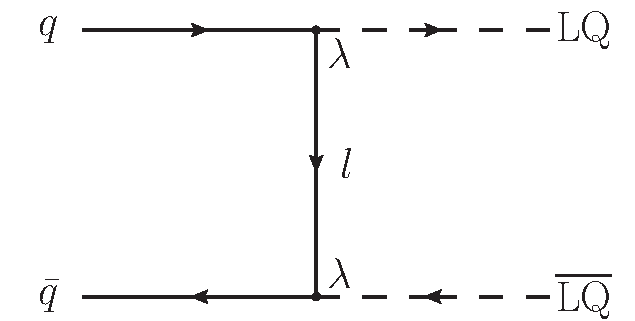
\includegraphics[width=0.49\textwidth]{figures/LO_FD_LQ_pair_b.pdf}
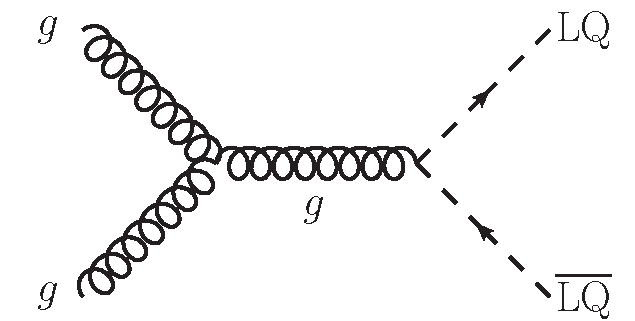
\includegraphics[width=0.49\textwidth]{figures/LO_FD_LQ_pair_c.pdf}
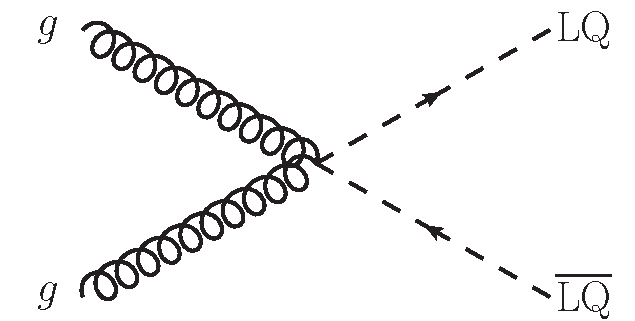
\includegraphics[width=0.49\textwidth]{figures/LO_FD_LQ_pair_d.pdf}
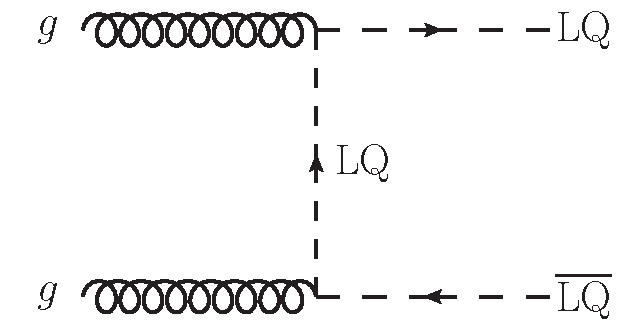
\includegraphics[width=0.49\textwidth]{figures/LO_FD_LQ_pair_e.pdf}
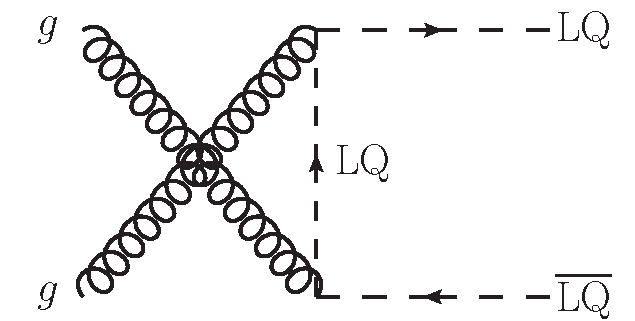
\includegraphics[width=0.49\textwidth]{figures/LO_FD_LQ_pair_f.pdf}
\caption{The LO Feynman diagrams for leptoquark pair production from quark-antiquark annihilation (top) and gluon-gluon fusion (middle, bottom).}
\label{fig:lq-diagrams}
\end{center}
\end{figure}

\begin{figure}[hbt]
\begin{center}
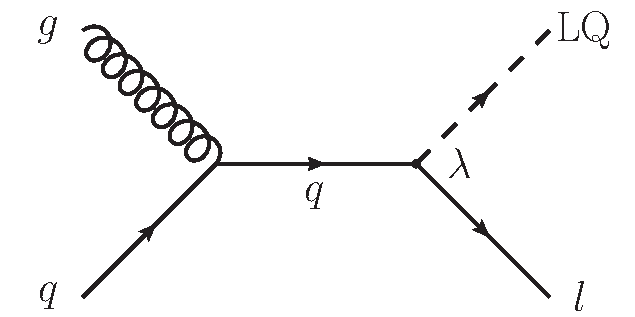
\includegraphics[width=0.49\textwidth]{figures/LO_FD_single_LQ_a.pdf}
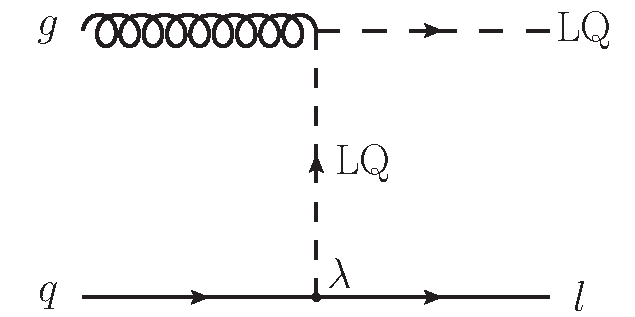
\includegraphics[width=0.49\textwidth]{figures/LO_FD_single_LQ_b.pdf}
\caption{The LO diagrams for single leptoquark production from quark-gluon scattering. The LQ is produced in association with a lepton.}
\label{fig:lq-single}
\end{center}
\end{figure}

Table \ref{tab:lq-xsec} lists the pair production cross sections for a range of scalar leptoquark masses. They have been calculated using the CTEQ6 parton distribution functions (PDFs) \cite{CTEQ6r1,CTEQ6r2} with $K$-factors applied to include NLO corrections from QCD \cite{LQxsec}. Theoretical uncertainties are calculated by propagating the PDF uncertainty and varying the factorization/renormalization scale $\mu$ from $\mu=\MLQ/2$ to $\mu=2\MLQ$. These cross sections are sensitive only to the leptoquark mass and spin, so they are largely model-independent. For vector leptoquarks, the cross sections may be modified by anomalous triple and quartic gauge couplings. The cross sections for vector leptoquarks are typically larger than the cross sections for scalar leptoquarks. The decay widths for scalar and vector leptoquarks can be calculated according to Eqs. \eqref{eq:SLQ-width} and \eqref{eq:VLQ-width}, respectively \cite{BRW}:
\begin{align}
\label{eq:SLQ-width} \Gamma_{S} &= \sum_{i}{\frac{\lambda_{i}^{2}}{16\pi}\MLQ}, \\
\label{eq:VLQ-width} \Gamma_{V} &= \sum_{i}{\frac{\lambda_{i}^{2}}{24\pi}\MLQ}.
\end{align}
Equations \eqref{eq:SLQ-width} and \eqref{eq:VLQ-width} sum over all Yukawa couplings for a given leptoquark. Given the limits on $\lambda$ discussed above, leptoquarks accessible at the LHC with a single Yukawa coupling can be expected to have a fractional decay width of less than 0.1--0.2\%.

\begin{table}[htb]
\begin{center}
{\footnotesize
\begin{tabular}{|l||c|c||c|c|}
\hline
$\MLQ$ $[\GeVns]$ & $\sigma (\mu = \MLQ)$ [pb] & $\delta (\text{PDF})$ [pb] & $\sigma (\mu = \MLQ/2)$ [pb] & $\sigma (\mu = 2\MLQ)$ [pb] \\
\hline
\hline
 200 & 17.4 & 1.24 & 15.0 & 19.7  \\
 250 & 5.26 & 0.487 & 4.54 & 5.94  \\
 300 & 1.89 & 0.214 & 1.63 & 2.13  \\
 350 & 0.77 & 0.102 & 0.663 & 0.866  \\
 400 & 0.342 & 0.052 & 0.295 & 0.385  \\
 450 & 0.163 & 0.0278 & 0.14 & 0.183  \\
 500 & 0.082 & 0.0155 & 0.0704 & 0.0922  \\
 550 & 0.0431 & 0.00893 & 0.037 & 0.0485  \\
 600 & 0.0235 & 0.0053 & 0.0201 & 0.0265  \\
 650 & 0.0132 & 0.00322 & 0.0113 & 0.0149  \\
 700 & 0.00761 & 0.002 & 0.00648 & 0.00858  \\
 750 & 0.00448 & 0.00126 & 0.00381 & 0.00506  \\
 800 & 0.00269 & 0.00081 & 0.00228 & 0.00304  \\
 850 & 0.00164 & 0.000527 & 0.00139 & 0.00186  \\
 900 & 0.00101 & 0.000347 & 0.000856 & 0.00115  \\
 950 & 0.000634 & 0.000231 & 0.000534 & 0.000722  \\
 1000 & 0.000401 & 0.000155 & 0.000337 & 0.000458  \\
\hline
\end{tabular}
}
\caption{The pair production cross sections for a range of scalar leptoquark masses at $\sqrt{s}=8\TeV$. Theoretical uncertainties from the PDFs and from varying the factorization/renormalization scale $\mu$ from $\mu=\MLQ/2$ to $\mu=2\MLQ$ are indicated.}
\label{tab:lq-xsec}
\end{center}
\end{table}

In this dissertation, a search is performed for pair production of scalar leptoquarks decaying to third generation fermions. The symbol $\mathcal{B}$ is used for the branching fraction for the decay $\text{LQ} \rightarrow \tau \cPqb$. Because they are pair produced, this results in a final state with two tau leptons and two bottom quarks. One tau lepton is required to decay leptonically: $\tau \rightarrow \ell \overline{\nu_{\ell}} \nu_{\tau}$, where $\ell$ can be a muon or an electron, which are collectively called light leptons. The other tau lepton is required to decay hadronically, denoted as \tauh; see Sec. \ref{sec:hpstau} for more information about hadronic decays of tau leptons. These decays result in two channels based on the leptonic decay of the tau, which are labeled as \etau and \mutau, or collectively \ltau when the light lepton flavor is unimportant. Both bottom quarks hadronize into b-jets, as described in Sec. \ref{sec:b-tagging}. Currently, the strongest mass limits on such third-generation scalar leptoquarks come from direct searches. Assuming $\mathcal{B}=100\%$, the lower limit is approximately 530\GeV, set by both the CMS \cite{CMSLQ3} and ATLAS \cite{ATLASLQ3} experiments using 4.7--4.8\fbinv of data from $\Pp\Pp$ collisions with $\sqrt{s}=7\TeV$. Indirect limits from low-energy processes are discussed in Refs. \cite{ModelIndLQ,Leurer:1993em, MuchAdo, LQreview}. Though this search does not consider vector leptoquarks explicitly, scalar and vector leptoquarks tend to have similar angular distributions. Combined with the larger cross section for vector leptoquarks, this implies that the same search can set higher mass limits on vector leptoquarks, as shown in Ref. \cite{CMSLQ3} for the 7\TeV data.

%talk about reinterpreted search to cover low B?

%\stepcounter{sectionprime}
\section{R-Parity Violating Supersymmetry
\label{sec:RPVSUSY}}

Supersymmetry proposes a symmetry between bosons and fermions. Such a symmetry appeals to mathematical considerations in quantum field theory by simplifying many calculations \cite{Peskin}. However, the primary motivation for a theory of SUSY with effects at the electroweak scale and therefore accessible at the LHC is the hierarchy problem. The mass of the Higgs boson, experimentally measured as $M_{\PH} = 125\GeV$, is theoretically sensitive to quantum corrections via loop diagrams from any particle that couples to it. This sensitivity arises due to the scalar nature of the Higgs boson, which means that there is no symmetry available to protect its mass value. Therefore, precise cancellations must occur among the various quantum corrections to produce such a small mass value, relative to the expected energy scales of new physics. Any BSM theory lacking a simple mechanism to produce such cancellations must undergo unnatural fine-tuning in order to arrive at the correct value of $M_{\PH}$. The following discussion of supersymmetry is drawn primarily from Ref. \cite{Primer}.

The Higgs mass parameter $m_{\PH}^{2}$ appears in the Higgs potential:
\begin{equation}
V = m_{\PH}^{2}|\PH|^{2} + \lambda_{\PH}|\PH|^{4}.
\end{equation}
Consider the one-loop contribution to $m_{\PH}^{2}$ from a fermion $f$ which has a Yukawa coupling to the Higgs field, $-y_{f} \overline{f}_{L} \PH f_{R}$. The correction term in the mass parameter calculation can be written as follows:
\begin{equation}
\Delta_{f} m_{\PH}^{2} = -\frac{|y_{f}|^{2}}{8\pi^{2}}\Lambda_{\text{UV}}^{2} + \cdots. \label{eq:DMH-fermion}
\end{equation}
The factor $\Lambda_{\text{UV}}$ is the cutoff scale used to handle the ultraviolet divergence in the loop integral through regularization. This cutoff scale is typically related to the energy scale of new physics, e.g. the GUT scale or Planck scale. Even if the cutoff scale is small, the contribution to the Higgs mass from any new heavy fermion will be proportional to its Yukawa coupling $y$, which could itself be large. Similarly, consider the one-loop contribution from a scalar boson $S$ with a coupling to the Higgs written as $-y_{S} |\PH|^{2} |S|^{2}$, which produces a correction term:
\begin{equation}
\Delta_{S} m_{\PH}^{2} = \frac{y_{S}}{16\pi^{2}}\Lambda_{\text{UV}}^{2} + \cdots. \label{eq:DMH-scalar}
\end{equation}
Both one-loop diagrams are shown in Fig. \ref{fig:higgs-cancel}. The leading terms of Eqs. \eqref{eq:DMH-fermion} and \eqref{eq:DMH-scalar} have opposite signs, which suggests that the two terms could cancel if there were two scalars, one left-handed and one right-handed, for each fermion, with $y_{S} = |y_{f}|^2$.

\begin{figure}[hbt]
\begin{center}
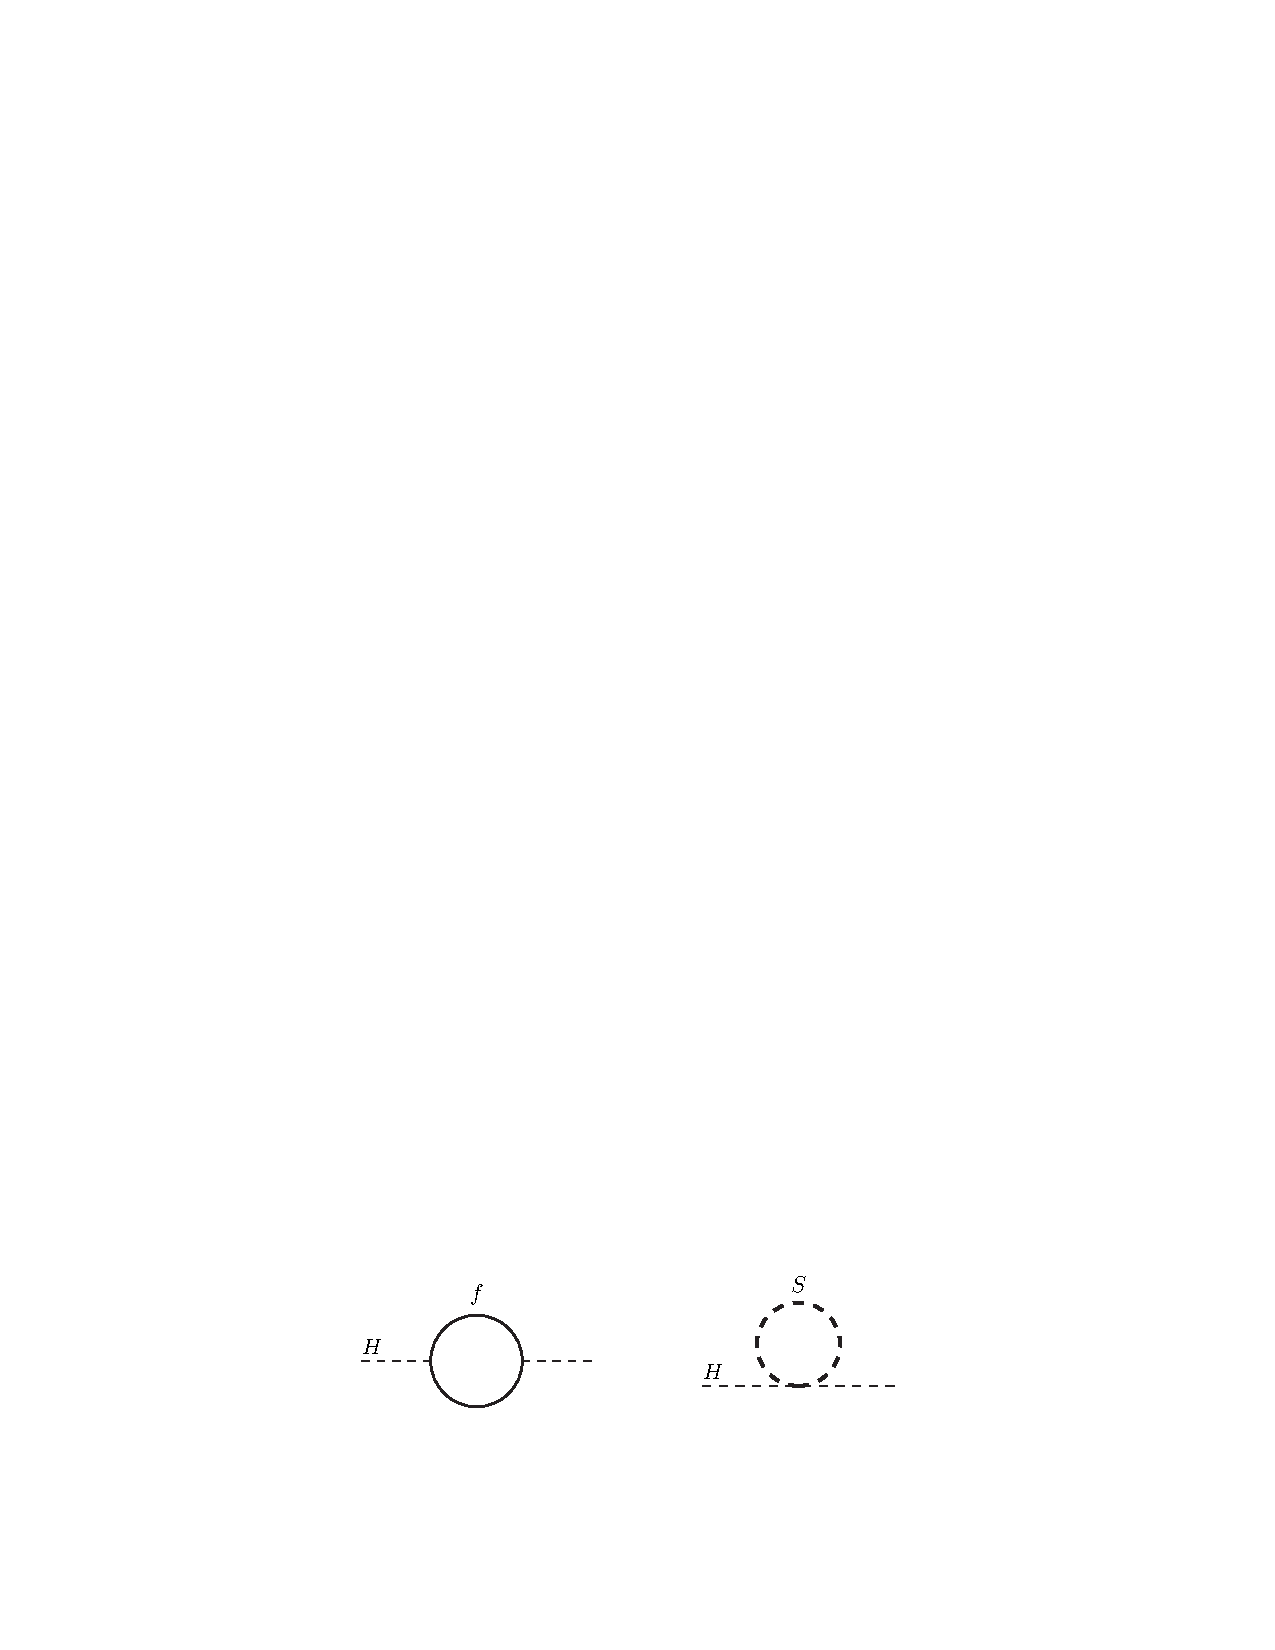
\includegraphics[width=0.95\textwidth]{figures/9709356v6-higgs-cancel.pdf}
\caption{One-loop diagrams for contributions to the Higgs mass parameter $m_{\PH}^{2}$ from a fermion $f$ (left) and a scalar $S$ (right) \cite{Primer}.}
\label{fig:higgs-cancel}
\end{center}
\end{figure}

This observation motivates SUSY as an extension of the standard model. While many formulations of SUSY exist, it is instructive to consider the minimal supersymmetric model (MSSM) to understand the fundamental components of the class of SUSY theories. SM particles are paired with new particles called superpartners with a spin difference of 1/2; SM fermions have scalar boson superpartners and SM bosons have spin-1/2 fermion superpartners. The scalar superpartners are named after the corresponding SM fermions with the prefix ``s-'', e.g. squarks and sleptons. The fermionic superpartners are named after the corresponding SM bosons with the suffix ``-ino'', e.g. higgsinos and gauginos. The symbols for superpartners are indicated by a tilde $\widetilde{\hphantom{H}}$. SM particles and their superpartners are arranged together in supermultiplets which extend the multiplets listed in Table \ref{tab:q-num}. Chiral supermultiplets contain scalar bosons and spin-1/2 fermions, while gauge supermultiplets contain spin-1/2 fermions and vector bosons. The superpartners possess the same quantum numbers as the corresponding SM particles, except for spin.

The Higgs boson, as a scalar, therefore becomes part of a chiral supermultiplet with weak hypercharge values $Y = \pm 1/2$. However, the existence of the corresponding chiral higgsinos creates new triangle gauge anomalies which must be cancelled to preserve the consistency of the theory. In addition, the weak hypercharge values of the Higgs supermultiplet restrict the possible Yukawa interactions with the other chiral supermultiplets, which are necessary for spontaneous fermion masses. For both of these reasons, the MSSM contains two Higgs doublets, conventionally labeled \Hone and \Htwo to indicate their couplings to up-type quarks or down-type quarks and charged leptons, respectively. Each Higgs doublet has its own VEV, labeled $v_{\cPqu}$ and $v_{\cPqd}$, respectively. The angle $\beta$ is defined as $\text{tan}(\beta) = v_{\cPqu}/v_{\cPqd}$, with each VEV taken as a component of a single value $v$.

Given these details, the superpotential of the MSSM, $W_{\text{MSSM}}$, contains these terms:
\begin{equation}
W_{\text{MSSM}} = y_{\cPqu,ij}\PU_{i}^{c}\PQ_{j}\Hone + y_{\cPqd,ij}\PD_{i}^{c}\PQ_{j}\Htwo + y_{\Pe,ij}\PE_{i}^{c}\PL_{j}\Htwo + \mu \Hone \Htwo. \label{eq:WMSSM}
\end{equation}
Equation \eqref{eq:WMSSM} is written in terms of superfields. $\PU$ is the up-type quark singlet superfield; $\PD$ is the down-type quark singlet superfield; $\PQ$ is the quark doublet superfield; $\PE$ is the charged lepton singlet superfield; and $\PL$ is the lepton doublet superfield. The Yukawa couplings $y$ are labeled by the fermion type $\cPqu$, $\cPqd$, or $\Pe$ with generation indices $i$, $j$. As an example, the top quark Yukawa coupling is $y_{\cPqu,33} = y_{\cPqt}$. The higgsino mass parameter is denoted as $\mu$.

The superpotential is limited to these terms by requiring the conservation of $R$-parity. The quantity $R$ is related to the baryon and lepton numbers as well as the particle spin $S$ and may be defined in two equivalent ways \cite{Barbier}, as shown in Eq. \eqref{eq:Rdef}. Equation \eqref{eq:Rparity} defines $R$-parity based on $R$.
\begin{align}
R &= 3B+L+2S = 3(B-L)+2S, \label{eq:Rdef} \\
R_{p} &= (-1)^{R}. \label{eq:Rparity}
\end{align}
All SM particles have $R_{p} = +1$, while all superpartners have $R_{p} = -1$. If $R$-parity is conserved, interactions which violate lepton or baryon number are not allowed. Notably, the lightest supersymmetric particle must be stable in order to conserve $R$-parity in the decays of SUSY particles. In many models, the LSP is the lightest neutralino, a state created by mixing between the neutral higgsinos and gauginos due to EWSB. As a weakly interacting massive particle, the neutralino LSP is a promising candidate for WIMP dark matter.

If supersymmetry were unbroken, superpartners would have the same masses as their corresponding SM particles and would already have been detected. Therefore, there must be some mechanism responsible for breaking supersymmetry. In order for broken SUSY to continue to solve the hierarchy problem, it must preserve the conditions such as $y_{S} = |y_{f}|^2$ that lead to natural cancellations in the Higgs mass correction terms. So-called ``soft'' supersymmetry breaking accomplishes this by separating the Lagrangian into two separate terms:
\begin{equation}
\mathcal{L} = \mathcal{L}_{\text{SUSY}} + \mathcal{L}_{\text{soft}},
\end{equation}
where $\mathcal{L}_{\text{SUSY}}$ is made up of the SUSY-preserving terms, including the Yukawa interactions from the superpotential as well as the gauge interactions, and $\mathcal{L}_{\text{soft}}$ is made up of the SUSY-violating terms. The contributions to $\mathcal{L}_{\text{soft}}$ must be only mass terms and couplings whose parameters have positive mass dimension. These include triple-scalar interactions between two sfermions and a Higgs, such as $a_{\cPqu,ij} \sUp_{i}^{c} \sQua_{j} \Hone$, where $a_{\cPqu,ij}$ are the soft couplings for those interactions. All such soft couplings are either at or below the mass scale $m_{\text{soft}}$, which is expected to be around the TeV scale from hierarchy problem considerations.

In general, the soft SUSY breaking terms can introduce FCNCs and charge-parity (CP) violation that are limited by precision measurements. These limits can be avoided by assuming the sfermion masses are universal; in other words, all sfermions should have the same mass regardless of flavor. This ``flavor-blindness'' eliminates mixing between flavors, and, as a bonus, greatly reduces the number of free parameters in the MSSM. The first- and second-generation sfermions possess flavor-blind universal masses. However, in the third generation, the sfermion masses can differ from the other two generations. In quantum field theory calculations, the couplings and mass parameters are treated as running factors which change based on renormalization group (RG) equations. These RG equations lead to corrections which tend to be small for Yukawa interactions, except for third generation particles, which have relatively large Yukawa couplings. In addition, at low energy scales, the slepton masses may deviate from the squark masses due to the different running behaviors of their respective couplings. The effects of RG evolution in SUSY on the gauge couplings for the three fundamental forces significantly aid grand unification, which is another motivation for SUSY.

The concept of naturalness, described in Ref. \cite{NaturalSUSY}, requires the third-generation sfermion masses to be relatively light, while the other superpartners may be heavy. The tree level relationship $M_{\Z}^{2} \propto |\mu|^{2} + |m_{\Hone}^{2}|$ implies that the superpartners with the largest contributions to $\mu$ and $m_{\Hone}^{2}$ must have masses near the electroweak scale. This applies especially to the higgsinos, whose masses are constrained by $\mu$, and to the top squark, whose partner the top quark generates the largest correction to $m_{\Hone}^{2}$. This consideration also applies to some extent to the other third-generation sfermions and the gluino. In addition, because the top squark masses are not flavor-blind, the mass eigenstates can involve significant mixing between the chiral eigenstates. The top squark mass matrix is written as follows:
\begin{equation}
\mathbf{m_{\sTop}^{2}} =
\begin{pmatrix}
m_{\PQ 3}^{2} + m_{\cPqt}^{2} + \Delta_{\sUp_{L}} & v(a_{\cPqt}^{\ast}\text{sin}(\beta) - \mu y_{\cPqt}\text{cos}(\beta)) \\
v(a_{\cPqt}\text{sin}(\beta) - \mu^{\ast} y_{\cPqt}\text{cos}(\beta)) & m_{\PU 3}^{2} + m_{\cPqt}^{2} + \Delta_{\sUp_{R}}
\end{pmatrix}.
\end{equation}
The terms $\Delta_{\sUp_{L}}$ and $\Delta_{\sUp_{R}}$ arise via hyperfine splitting from quartic interactions and are defined in Ref. \cite{Primer}. When this mass matrix is diagonalized, a large mixing angle typically occurs because of the off-diagonal entries, which contain terms involving the large top Yukawa coupling and soft coupling. This means that one top squark mass eigenstate will be lighter than the other, and in fact it will be the lightest squark. This mass splitting, together with the general consideration of naturalness that implies a light top squark mass, suggests that top squarks are likely to be accessible at the LHC.

In $R$-parity conserving (RPC) SUSY, all decays of superpartners eventually produce at least one LSP. As a weakly interacting particle, the LSP will escape a particle detector without interacting, leading to events with signatures including large missing transverse energy or \met. The precise details of the production and decay of SUSY particles depend on which model is considered. This section has focused on the MSSM, but many variations of this model exist. These include, but are not limited to \cite{PDG}: the constrained MSSM, in which there are only five parameters: the sfermion mass $m_0$, the gaugino mass $m_{1/2}$, the soft parameter scale $A_{0}$, $\text{tan}(\beta)$, and $\mu$; the phenomenological MSSM, which uses experimental limits to restrict the number of free parameters to ${\sim}19$; and the next-to-MSSM, which introduces a gauge singlet field to explain the electroweak-scale value of $\mu$ \cite{NMSSM}. In order to produce results with the broadest possible applicability, the CMS experiment uses simplified models, sometimes called decoupled models, in which the SUSY particles not under direct consideration are assumed to have masses too large to contribute significantly to the interactions. The latest results from the broad program of SUSY searches at the CMS experiment with $\sqrt{s}=8\TeV$ are summarized in Fig. \ref{fig:cms-susy-limits}. The requirements for naturalness introduced in Ref. \cite{NaturalSUSY}, which include top squark and bottom squark masses less than 500--700\GeV and gluino mass less than 900-1500\GeV, are very nearly excluded at this point. In addition, recent measurements of the decay $\Bz_{\cPqs} \rightarrow \mu^{+} \mu^{-}$ from the CMS \cite{CMS-BSmumu} and LHCb \cite{LHCb-BSmumu} experiments are in agreement with the SM prediction, further limiting the possible forms of SUSY, which would enhance this decay.

\afterpage{
\begin{landscape}
\begin{figure}%[hbtp]
\begin{center}
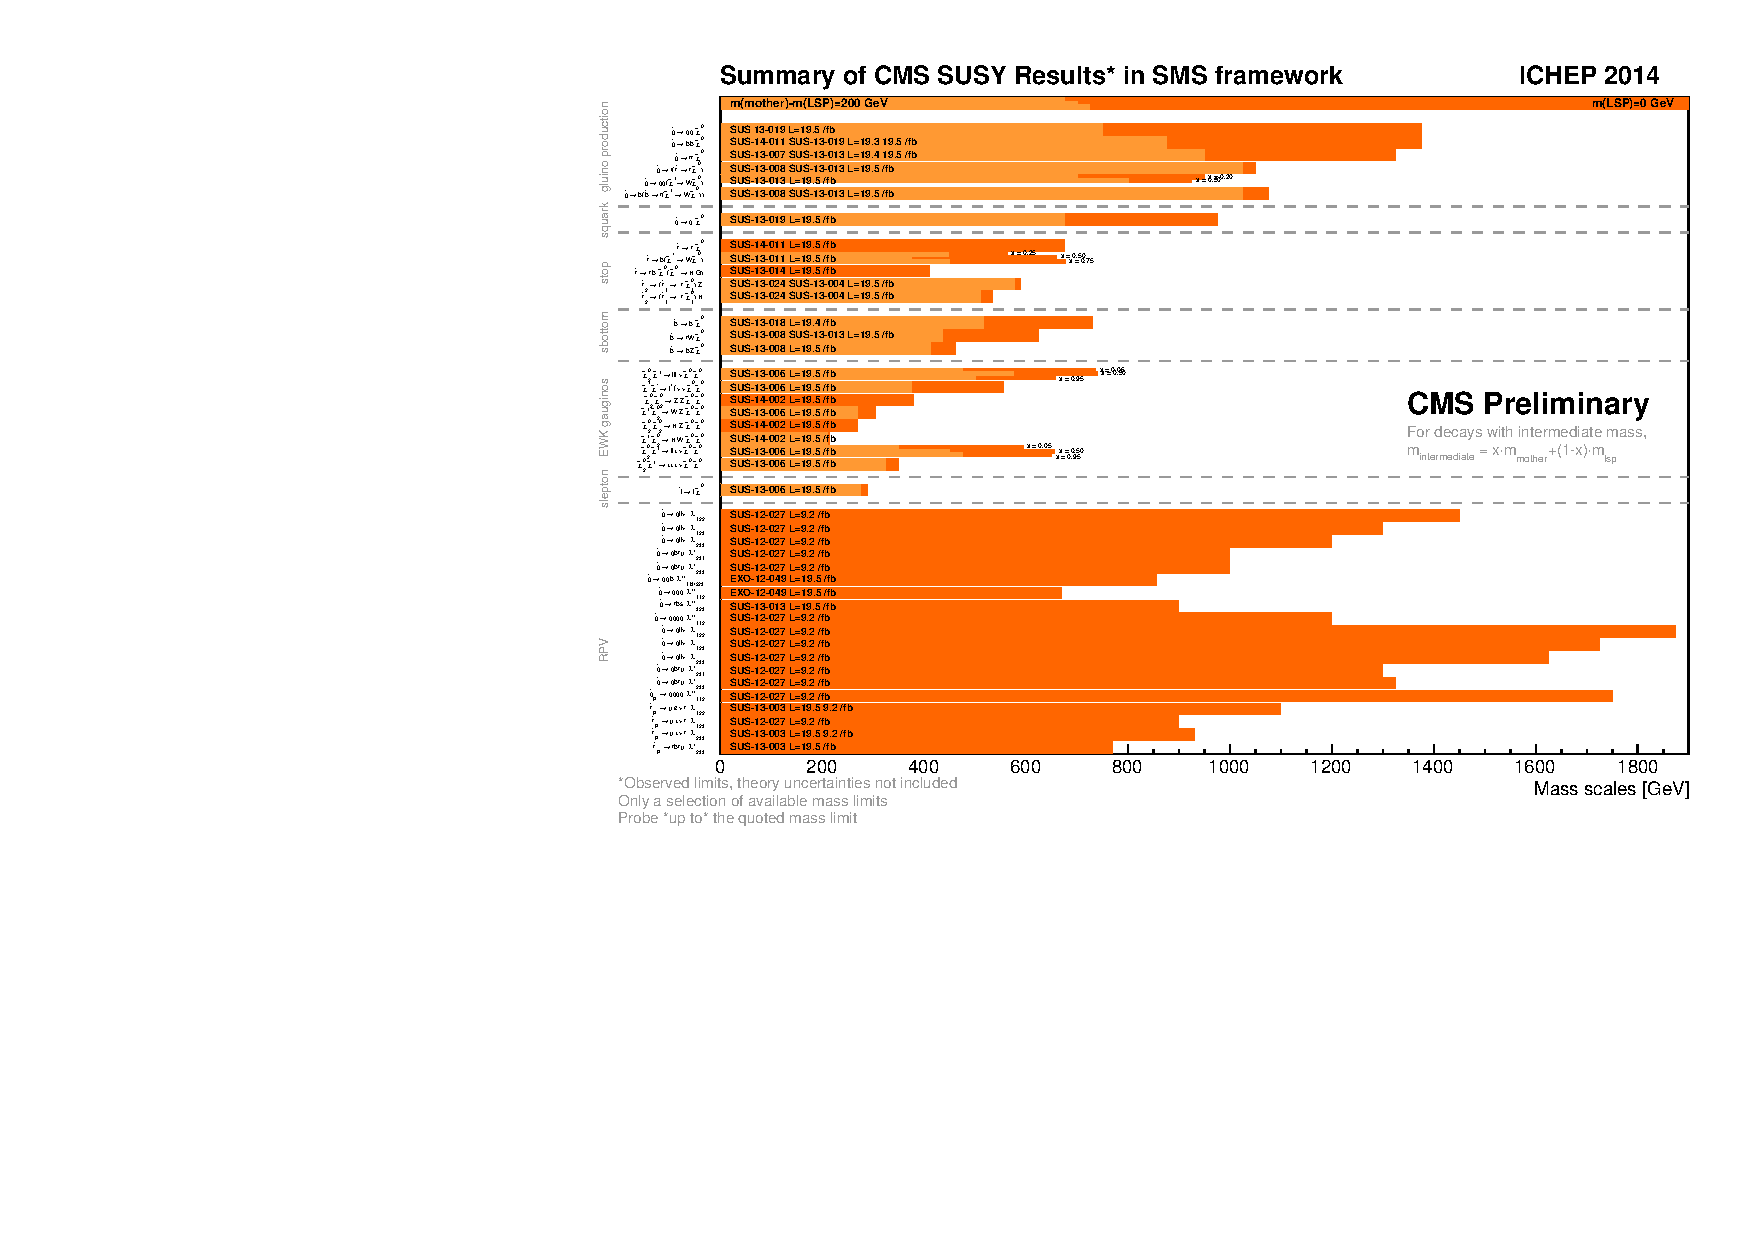
\includegraphics[height=350pt]{figures/barplot_ICHEP2014.pdf}
\caption{Summary of CMS exclusion limits for the masses of various SUSY particles with $\sqrt{s}=8\TeV$ \cite{CMS-SUSY-LIMITS}. These limits assume simplified models and unity branching fractions for the specified decays. Two scenarios are presented: the dark shades show $m(\text{LSP})=0$ and the light shades show $m(\text{mother})-m(\text{LSP})=0$.}
\label{fig:cms-susy-limits}
\end{center}
\end{figure}
\end{landscape}
}

The introduction of $R$-parity violating (RPV) terms in the SUSY Lagrangian is one way to evade these limits. If $R$-parity is violated, SUSY particles can decay to final states containing only SM particles, avoiding the characteristically large \met from the LSP, which is no longer stable. This generally eliminates the LSP as a dark matter candidate, making it a less popular option. However, RPV SUSY still solves the hierarchy problem and assists in grand unification. The possible RPV terms in the superpotential are \cite{Barbier}:
\begin{equation}
W_{\text{RPV}} = \frac{1}{2}\lambda_{ijk}\PL_{i}\PL_{j}\PE_{k}^{c} + \lambda_{ijk}^{\prime}\PL_{i}\PQ_{j}\PD_{k}^{c} + \frac{1}{2}\lambda_{ijk}^{\prime \prime}\PU_{i}^{c}\PD_{j}^{c}\PD_{k}^{c} + \mu_{i}\PL_{i}\Hone. \label{eq:WRPV}
\end{equation}
The different RPV coupling constants are denoted as $\lambda_{ijk}$, $\lambda^{\prime}_{ijk}$, $\lambda^{\prime \prime}_{ijk}$, and $\mu_{i}$, where $i$, $j$, and $k$ are generation indices. Figure \ref{fig:trilinear-RPV} shows the tree-level diagrams for the trilinear RPV couplings. As indicated by Fig. \ref{fig:trilinear-RPV} and the definition of $R$ in Eq. \eqref{eq:Rdef}, violating $R$ is equivalent to violating lepton number or baryon number. Scenarios which allow all of the RPV couplings produce large contributions to proton decay, due to the violation of both $B$ and $L$, and are therefore ruled out. Scenarios in which only a certain type of RPV coupling is allowed can still be viable.

\begin{figure}[hbt]
\begin{center}
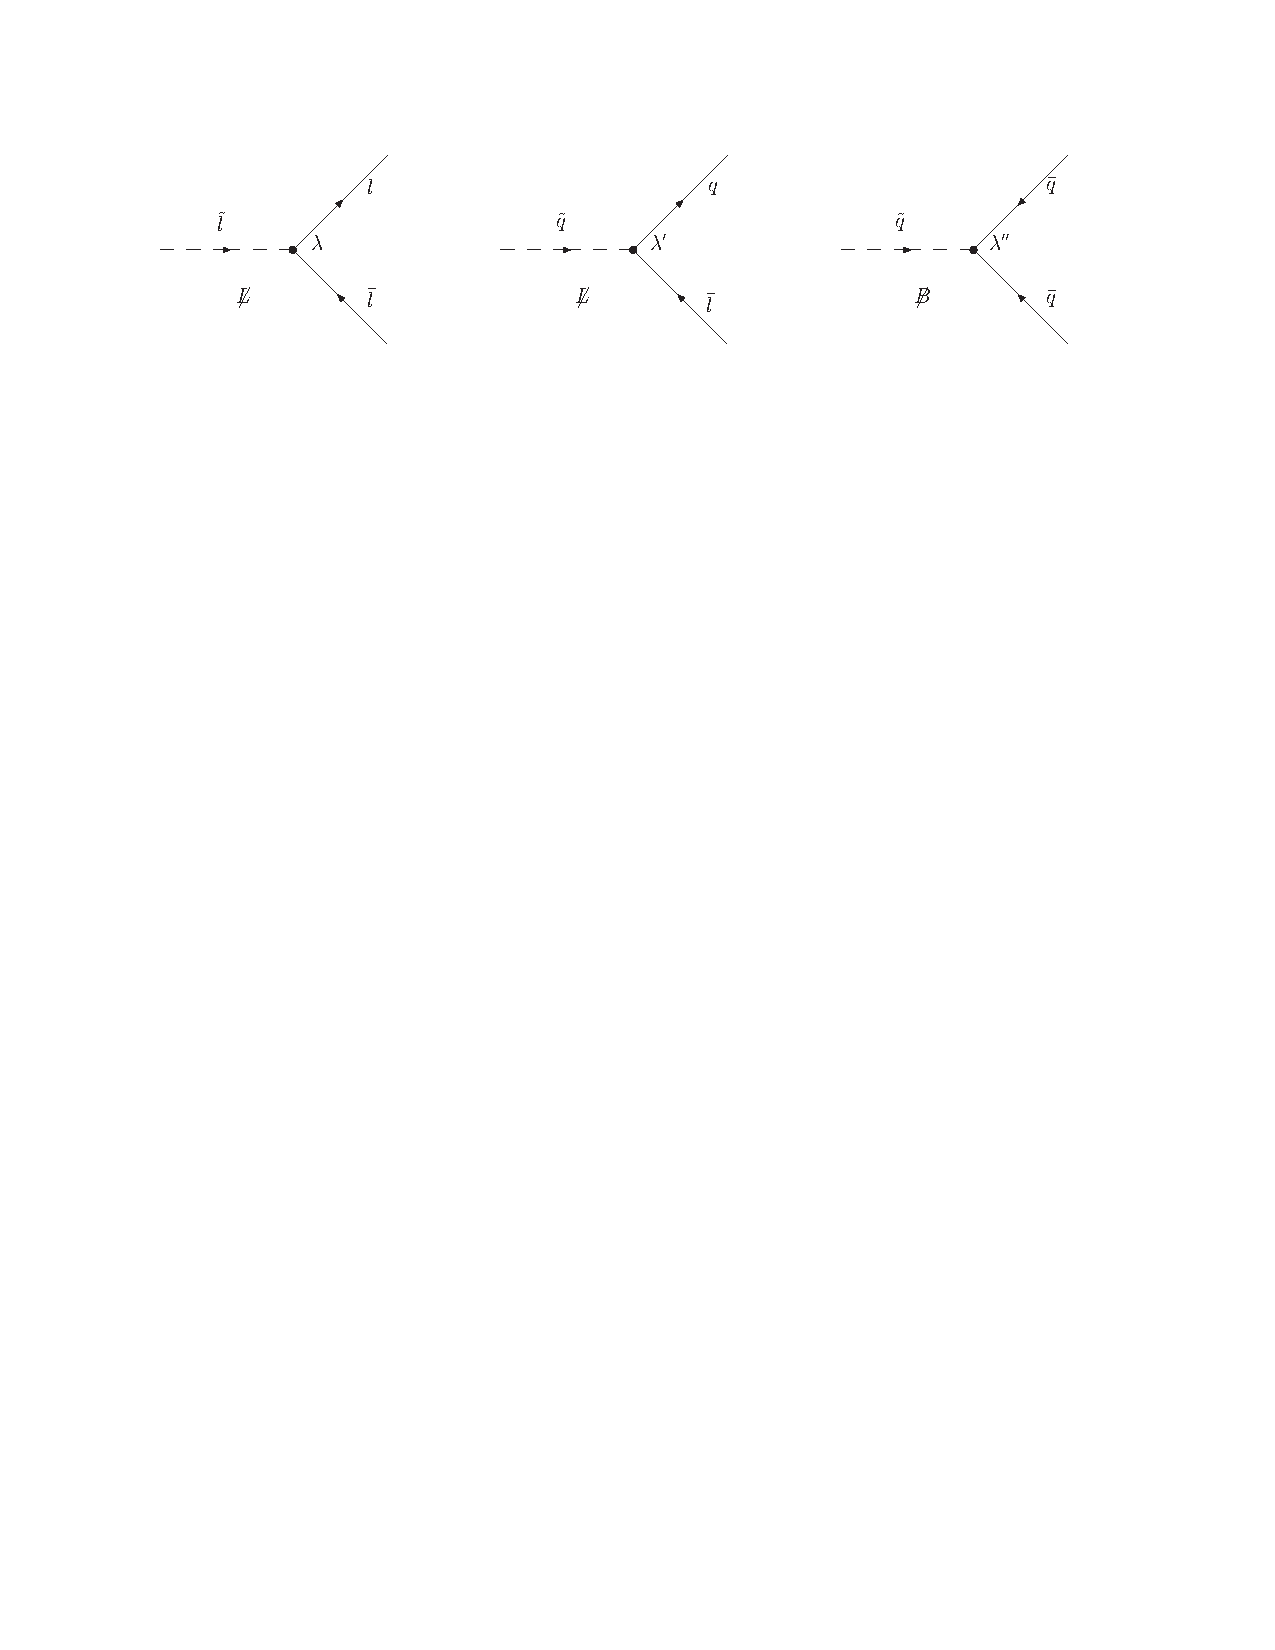
\includegraphics[width=0.95\textwidth]{figures/0406039v2_trilinear.pdf}
\caption{The LO diagrams for the three trilinear RPV couplings $\lambda$ (left), $\lambda^{\prime}$ (middle), and $\lambda^{\prime \prime}$ (right) \cite{Barbier}. These couplings violate lepton number, lepton number, and baryon number, respectively.}
\label{fig:trilinear-RPV}
\end{center}
\end{figure}

This dissertation considers the pair production of top squarks with two different RPV decays, using a decoupled model as described above. As a strongly-interacting scalar particle, the top squark has a production cross section that is identical to the leptoquark production cross section at leading order. In decoupled models, the cross section depends on the squark mass scale and the top squark mixing angle only at higher order, and the corrections from these terms amount to less than 2\% \cite{StopCrossSec}. The first decay considered is $\sTop \rightarrow \tau \cPqb$ via the coupling $\lambda_{333}^{\prime}$. The final-state signature and kinematic distributions of this signal are identical to those from the pair production of third-generation scalar leptoquarks, as described in Sec. \ref{sec:LQ}. Therefore, the results of the leptoquark search can be directly reinterpreted to apply to the $\lambda_{333}^{\prime}$ decay of top squarks.

In some natural SUSY models, if the higgsinos are lighter than the top squark, or if the RPV couplings that allow direct decays to SM particles are sufficiently small, the top squark decay may preferentially proceed via superpartners \cite{Jared}. This motivates the second search in the dissertation, which focuses on a scenario in which the dominant RPC decay of the top squark is $\sTop \rightarrow \chipm\cPqb$. This requires the mass splitting between the top squark and the chargino to be less than the mass of the top quark, so it is chosen to be 100\GeV. The chargino is assumed to be a pure higgsino and to be nearly degenerate in mass with the neutralino, with a decay $\chipm \rightarrow \sNu\tau^{\pm} \rightarrow \cPq\cPq\tau^{\pm}$. The decay of the sneutrino occurs via the RPV coupling $\lambda_{3jk}^{\prime}$, where the cases $j, k = 1, 2$ are considered. Such a signal can only be probed by searches that do not require large \met, as chiral suppression prevents the other possible decay of the chargino, $\chipm\to\nu\sTau$, from contributing to scenarios involving the $\lambda_{3jk}^{\prime}$ coupling.

The final state from pair production of top squarks undergoing this chargino-mediated RPV decay contains two tau leptons, two b-jets, and at least four additional jets. The search for the signal with this final state is called the top squark search, to distinguish it from the similar but not identical final state in the leptoquark search. As in the leptoquark search, the analysis is divided into two channels, \etau and \mutau, based on the required leptonic decay of one of the tau leptons. The symbol $\mathcal{B}$ in the top squark search is used to represent the branching fraction for the decay $\sTop \rightarrow \chipm\cPqb, \chipm \rightarrow \sNu\tau^{\pm} \rightarrow \cPq\cPq\tau^{\pm}$.  This dissertation presents the first search for the chargino-mediated $\lambda_{3jk}^{\prime}$ decay of the top squark.

%\renewcommand{\thesection}{\thechapter.\arabic{section}} % back to regular numbering